\documentclass[exa]{exercise_5.0}

\deadline{16.12.2024}

\begin{document}

\section{Verbindung mikroskopischer und makroskopischer
Größen}
Im NaCl-Kristall sind im Mittel genauso viele Natrium wie Chlor Atome. Die Anzahl an Elementarzellen $N$ kann dann auf zwei Wegen, entweder mit den Volumen oder den Massen, beschrieben werden: 
\begin{align*}
    N &= \frac{V}{a^3} 
    = \frac{M}z \frac1{m\sub{Na} + m\sub{Cl}}
    = \frac{N_A M}z\frac1{A\sub{Na} + A\sub{Cl}}\\\\
    \Aboxed{a &= \hug{\frac{z}{N_A \rho}(A\sub{Na} + A\sub{Cl})}^{\frac13} \approx 5.64\A}
\end{align*}

\section{Raumausfüllung in kubischen Gittern}
\subsection{\normalfont{\bf bcc}}
\begin{itemize}
    \item {\bf Anzahl der Atome in konventioneller Einheitszelle:} Es gibt acht Atome die an den Ecken zu einem achtel in der Zelle sind, und ein Atom im Zentrum. Insgesamt also zwei Atome pro Einheitszelle.
    \item {\bf Anzahl nächster Nachbarn:} Jedes Atom hat wie man der Skizze entnehmen kann acht nächste Nachbarn.
    \item {\bf Raumausfüllung:}
    \begin{align*}
        \frac{V\sub{atoms}}{V\sub{unit cell}}
        &= \frac{2\cdot \frac{4\pi}{3}R^3}{a^3}
        = \frac{2\cdot \frac{4\pi}{3}\cdot \hug{\frac12\sqrt{3\cdot (a/2)^2}}^3}{a^3}
        = \frac{3^{\frac12}\pi}{8}\approx 68.0\% 
    \end{align*}
\end{itemize}

\subsection{\normalfont{\bf fcc}}
\begin{itemize}
    \item {\bf Anzahl der Atome in konventioneller Einheitszelle:} Es gibt acht Atome die an den Ecken zu einem achtel in der Zelle sind, und sechs Atome auf den Seiten, die jeweils zur Hälfte in der Zelle sind. Insgesamt also $8\cdot 1/8 + 6\cdot1/2 = 4$ Atome pro Einheitszelle.
    \item {\bf Anzahl nächster Nachbarn:} Jedes Atom hat $3\cdot 4=12$ nächste Nachbarn.
    \item {\bf Raumausfüllung:}
    \begin{align*}
        \frac{V\sub{atoms}}{V\sub{unit cell}}
        &= \frac{4\cdot \frac{4\pi}{3}R^3}{a^3}
        = \frac{4\cdot \frac{4\pi}{3}\cdot \hug{\frac12\sqrt{2\cdot (a/2)^2}}^3}{a^3}
        = \frac{2^\frac12\pi}{6}\approx 74.0\% 
    \end{align*}
\end{itemize}

\section{Hexagonale Kristallstrukturen}
\subsection{}
Wie man in der Skizze sehen kann, reicht die grüne Zelle alleine nicht raus um durch reine Verschiebungen das Gitter zu rekonstruieren, da die pinken Bereiche nicht bedeckt werden können. Man muss also mindestens als Elementarzelle eine grüne mit einer pinken Zelle nehmen, um damit das Gitter vollständig aufgebaut werden kann. Die Skizze zeigt eine Zusammensetzung aus so definierten Elementarzellen, dessen Form wieder die der Elementarzelle gleicht. Die so entstehende Rekursionsvorschrift zur vervierfachung der lückenlos bedeckten Fläche beweist, dass die PEZ tatsächlich das Gitter vollständig aufbaut.   

Das in Abb. 2 gezeigte Gitter setzt sich dann zusammen aus drei PEZs.
\begin{figure}[H]
    \centering
    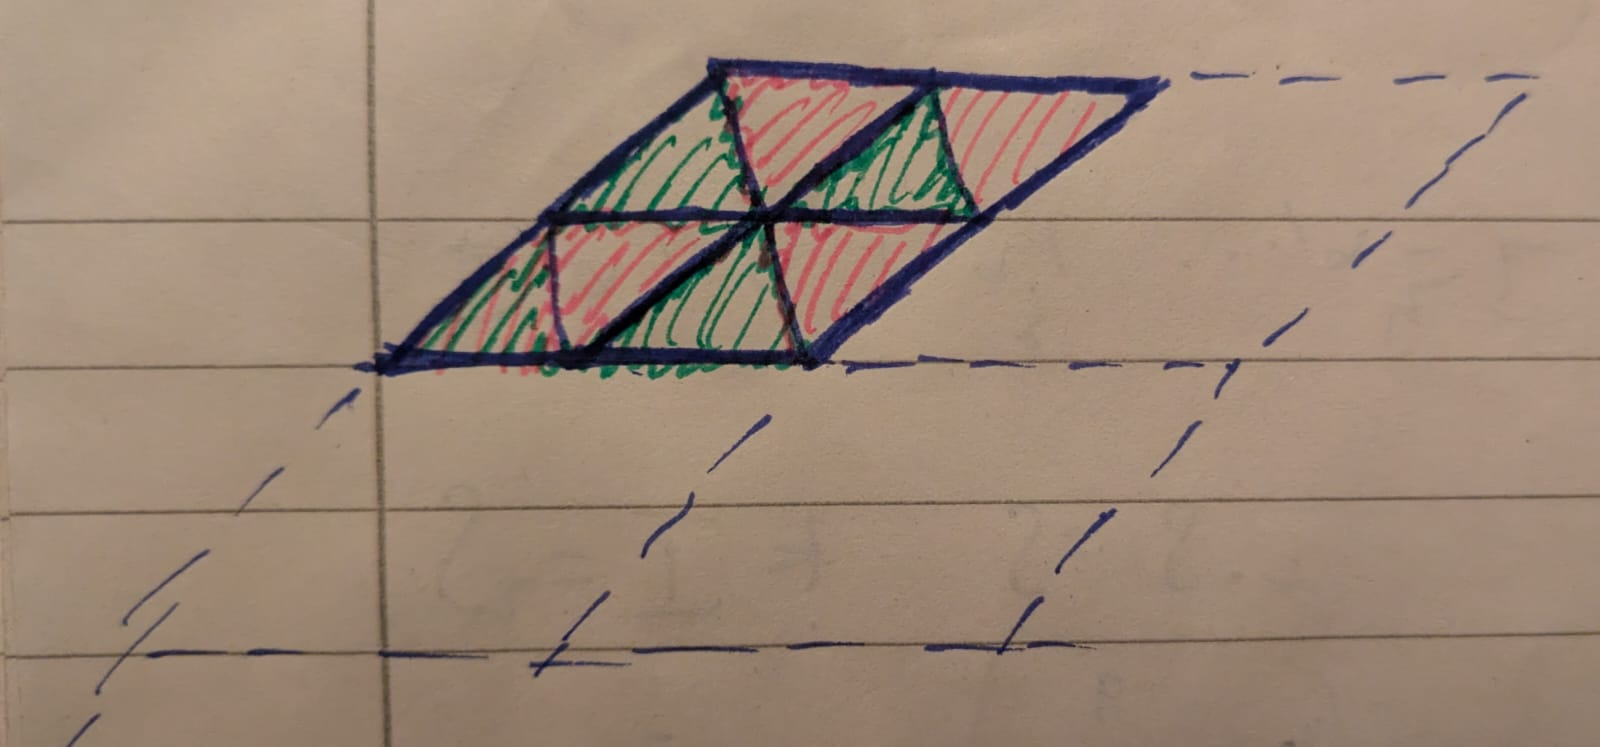
\includegraphics[width=.6\textwidth]{gitter.jpg}
    \caption{Skizze}
\end{figure}

\subsection{}
Eine PEZ darf per Definition nur ein Atom beinhalten, das in Abb. 2 abgebildete Gitter hat aber offensichtlich mehr. 

\subsection{}
\begin{align*}
    \frac{V\sub{atoms}}{V\sub{unit cell}}
        &= \frac{z\frac{4\pi}{3}R^3}{a h c}\\
        &= \frac{2\frac{4\pi}{3}(a/2)^3}{a\cdot \sqrt{a^2 - (a/2)^2}\cdot c}\\
        &= \frac{2\pi}{3\sqrt3} \frac ac\\
        &= \frac{2\pi}{3\sqrt3} \sqrt{\frac38}\note[siehe (d)]\\
        \Aboxed{\frac{V\sub{atoms}}{V\sub{unit cell}} &= \frac{\pi\sqrt 2}{6}\approx 74\%}
\end{align*}

\subsection{}
\begin{align*}
    c &= 2\cdot \sqrt{a^2 - \hug{\frac{a}{2\cos^230^\circ}}^2}\\
    \frac ca &= 2\cdot \sqrt{1 - \hug{\frac{1}{2\cos^230^\circ}}^2}\\
    &= 2\cdot \sqrt{1 - \hug{\frac{1}{3}}^2}\\
    \Aboxed{\frac ca&=\sqrt{\frac 83}}
\end{align*}

\section{N-zählige Drehachsen u. Translationssymmetrie}
Seien das Gitter $G$ und eine diskrete Drehung $R_n$ definiert als
\begin{align*}
    G &= \pug{n_1  a_1 + n_2  a_2: n_i\in\Z, \v a_i\in \C},\qquad R_n= e^{i\frac{2\pi}{n}}
\end{align*}
Betrachetet man für einen Gitterpunkt $p\in G$ die rotierten Gitterpunkte $R_n p$ und $R_n\inv p$, so müssen diese wieder in $G$ liegen. Für die Translationssymmetrie muss das Gitter wieder auf sich selbst abgebildet werden, wenn man einen beliebigen Gitterpunkt zuaddiert $G+p \equiv G$. Vor allem muss daher $R_n p + R\inv _n p\propto p$ auch wieder ein Gitterpunkt sein. Damit das möglich ist muss der resultierende Vektor ein ganzzahliges Vielfaches von $p$ sein: 
\begin{align*}
    m p &\peq R_n p + R\inv _n p\note m\in\Z\\
    &= \hug{e^{i\frac{2\pi}{n}} + e^{-i\frac{2\pi}{n}}}p\\
    m &= 2\cos\frac{2\pi}{n}
\end{align*}
Die einzigen Lösungen sind:
\begin{align*}
    \binom nm &= \binom{\pm 1}{2},\binom{\pm2}{-2},\binom{\pm 3}{-1},\binom{\pm4}{0}, \binom{\pm6}{1}
\end{align*}
Entsprechend den Rotationen um $\pm360^\circ, \pm180^\circ, \pm120^\circ,\pm90^\circ$ und $\pm60^\circ$.

\section{Leerstellenkonzentration in Aluminium}
Jeder Gitterplatz ist entweder eine Leerstelle oder nicht. Der Einfachheit halber sei angenommen, dass diese Besetzungen verschiedener Gitterplätze unabhängig voneinander stattfinden. Unter dieser Annahme wird die Entropie des Systems maximal wenn die Besetzungswahrscheinlichkeit eines jeden Gitterplatz Boltzmannverteilt ist. Sei die Energieskala so geeicht, dass ein besetzter Gitterplatz der Energie $0$ entspricht und eine Lücke der Energie $\Delta$. Dann ergibt sich für die Leerstellenkonzentration wenig überraschend eine Fermi-Dirac-Verteilung:
\begin{align*}
    Z &= \sum_n e^{-\beta E_n} = 1 + e^{-\beta \Delta}\\ 
    c_V(T) &= \frac{e^{-\beta\Delta }}{Z} = \frac1{e^{\beta \Delta} + 1}
\end{align*}
Die Energiedifferenz $\Delta$ ist dann:
\begin{align*}
    \Delta&= k_B T \ln\hug{\frac1{c_V}-1}
\end{align*}
Für Raumtempertur/Schmelztemperatur ergeben sich:
\begin{align*}
    \Delta_R &= 0.636\u{eV}, \qquad \Delta_M = 0.564 \u{eV}
\end{align*}


\section{Beugung mit Elektronen und Neutronen}
\subsection{}
Es gilt mit der de-Broglie-Wellenlänge $\lambda = \frac{h}{p}$:
\begin{align*}
    E &= \sqrt{m^2 c^4 + p^2 c^2}- mc^2
    = \sqrt{m^2 c^4 + \frac{h^2 c^2}{\lambda^2}} - mc^2
\end{align*}
Für die Massen von Elektron und Neutron ergeben sich:
\begin{align*}
    E_e &= 37.6\u{eV},\qquad E_n = 20.5\u{meV}
\end{align*}

\subsection{}
Es wird der Dulong-Petit-Grenzwert verwendet: 
\begin{align*}
    E &= \frac32 k_B T \ \Leftrightarrow \ T = \frac23 \frac{E}{k_B}
\end{align*}
Für Elektron und Neutron ergeben sich dann die folgenden Temperaturen:
\begin{align*}
    T_e &= 2.91\E{5}\u{K},\qquad T_n = 158\u{K}
\end{align*}

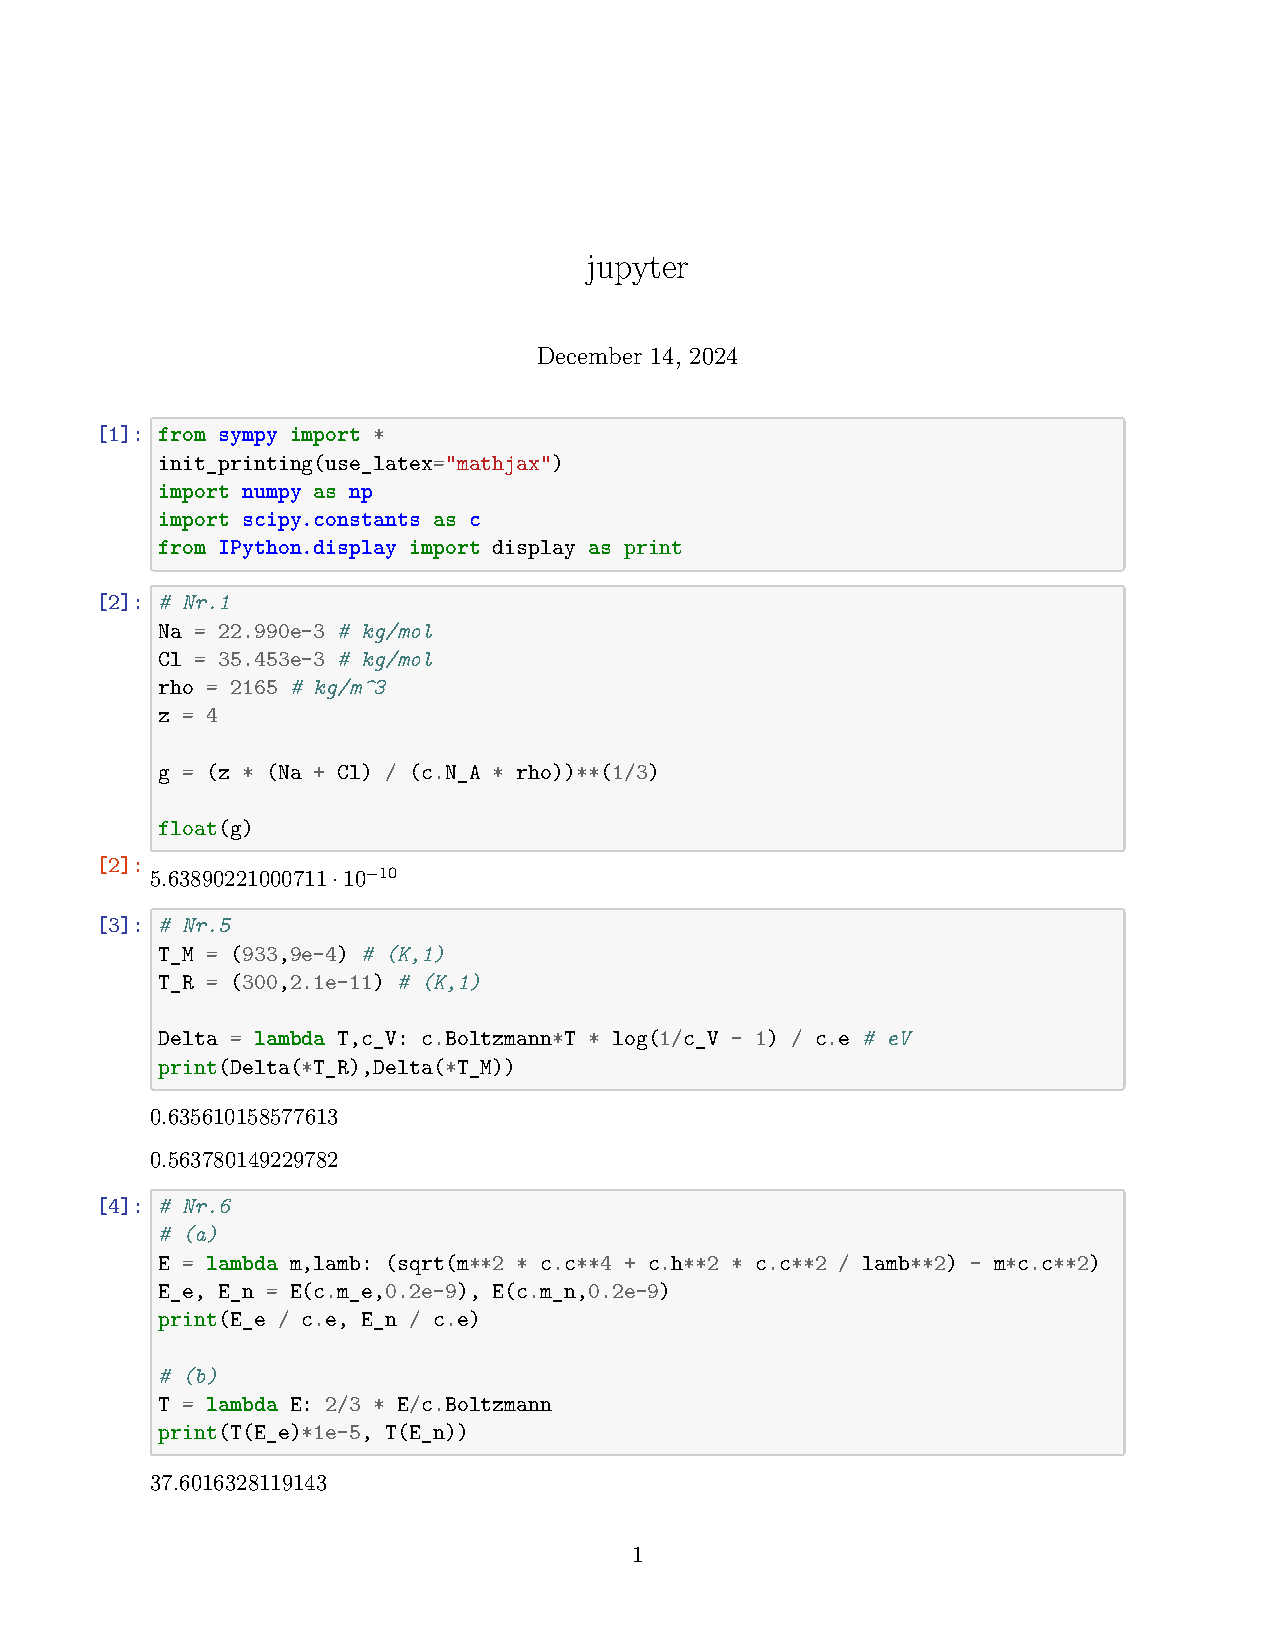
\includepdf[pages=-]{jupyter.pdf}

\end{document}